%Especificacion
\documentclass[12pt]{article}

%Paquetes
\usepackage[left=2cm,right=2cm,top=3cm,bottom=3cm,letterpaper]{geometry}
\usepackage{lmodern}
\usepackage[T1]{fontenc}
\usepackage[utf8]{inputenc}
\usepackage{hyperref}
\usepackage{float}
\usepackage{caption}
\usepackage[spanish,activeacute]{babel}
\usepackage{mathtools}
\usepackage{amssymb}
\usepackage{enumerate}
%\usepackage{tabularx}
%\usepackage{wasysym}
\usepackage{graphicx}
\usepackage{pmboxdraw}
\graphicspath { {pics/} }
%\usepackage{pifont}
%Preambulo
\title{Sistemas Operativos\\ Guía visual: Instalación de Minix}
\author{Andrea González Vargas\\Carlos Gerardo Acosta Hernández}
\date{Facultad de Ciencias UNAM \\ 2019-2}
\setlength\parindent{0pt}

\begin{document}
\maketitle

Antes de comenzar la instalación, descargar la imagen ISO de \texttt{Minix 3} en la página oficial\footnote{\url{https://wiki.minix3.org/doku.php?id=www:download:start}}:
\begin{figure}[H]
  \centering
  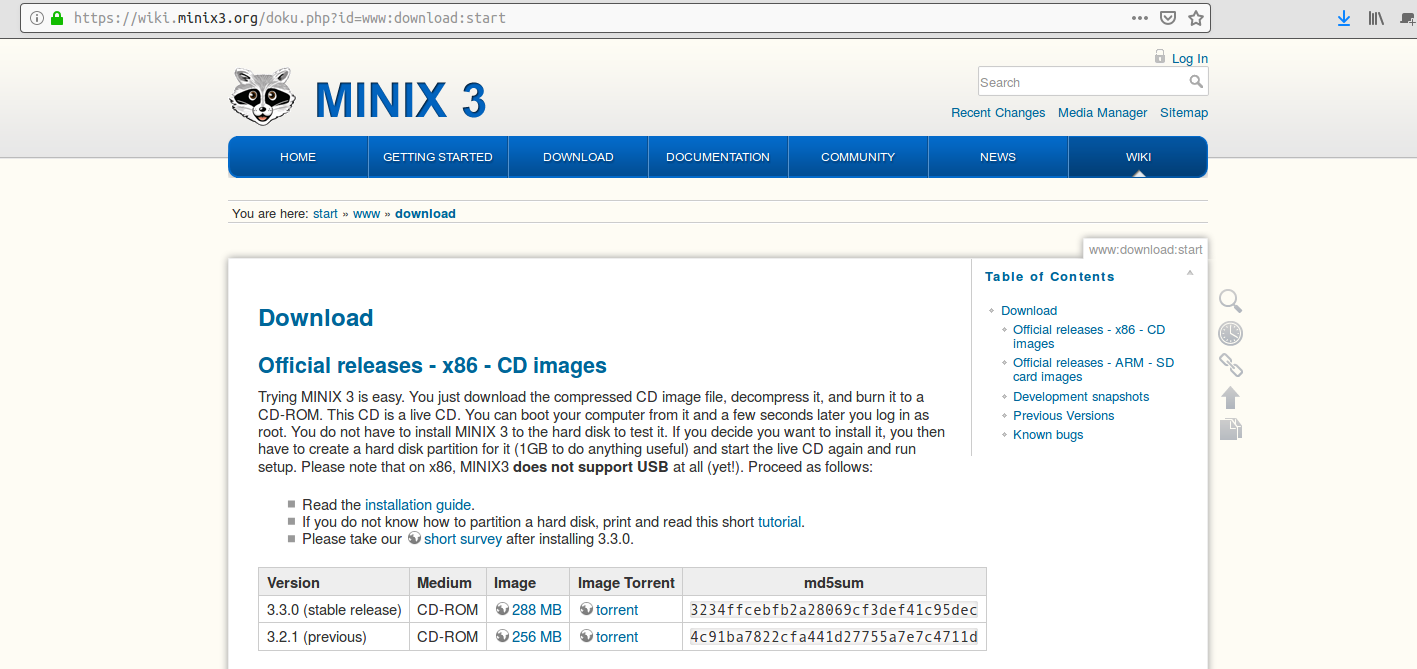
\includegraphics[width=\textwidth]{vm/min00.png}
  \caption{Página oficial de descarga de \texttt{Minix 3}}
\end{figure}

Proseguir a seguir las instrucciones del virtualizador que vaya a utilizarse (VMWare o VirtualBox):

\section{VMWare}

\subsection*{Preparación de la máquina virtual}

Crear una nueva máquina virtual accediendo a \textit{File $\rightarrow$ New\ Virtual\ Machine}.\\

Escoger la configuración de tipo \textit{Typical}.
\begin{figure}[H]
  \centering
  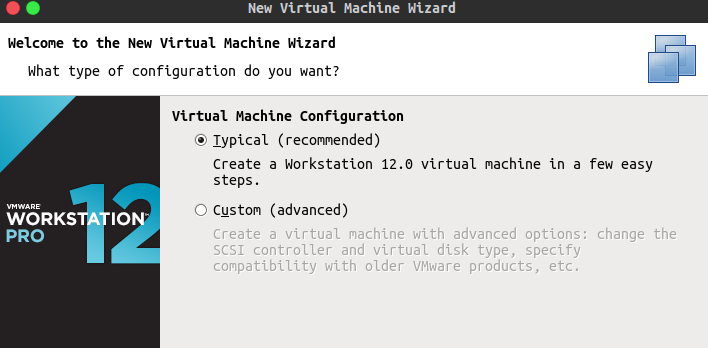
\includegraphics[width=0.6\textwidth]{vm/min01.png}
  \caption{Creación de nueva máquina virtual}
\end{figure}

Indicar que se instalará el sistema operativo después de la creación de la máquina virtual.
\begin{figure}[H]
  \centering
  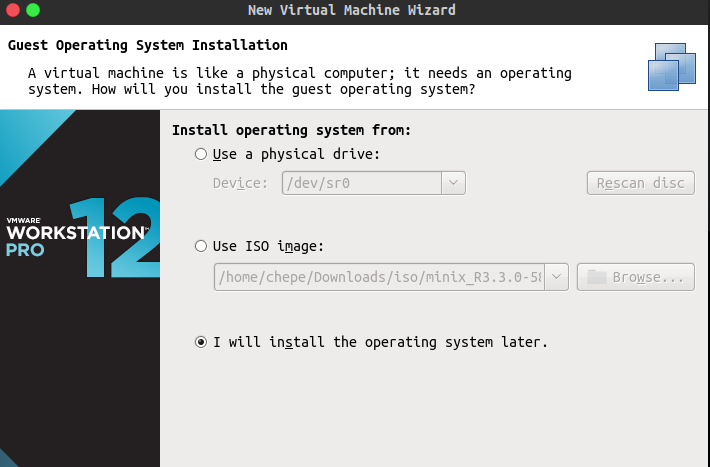
\includegraphics[width=0.6\textwidth]{vm/min02.png}
  \caption{Opciones de sistema operativo}
\end{figure}

Seleccionar \textit{Other} para el tipo de sistema operativo a instalar.
\begin{figure}[H]
  \centering
  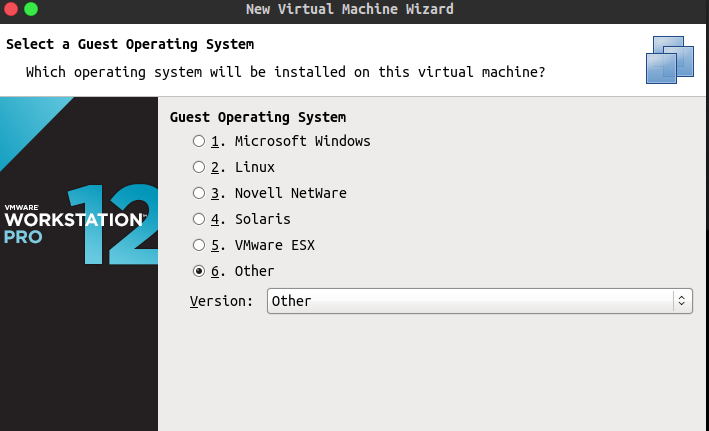
\includegraphics[width=0.6\textwidth]{vm/min03.png}
  \caption{Tipo de sistema operativo a instalar}
\end{figure}

Nombrar máquina e indicar la ruta de creación.
\begin{figure}[H]
  \centering
  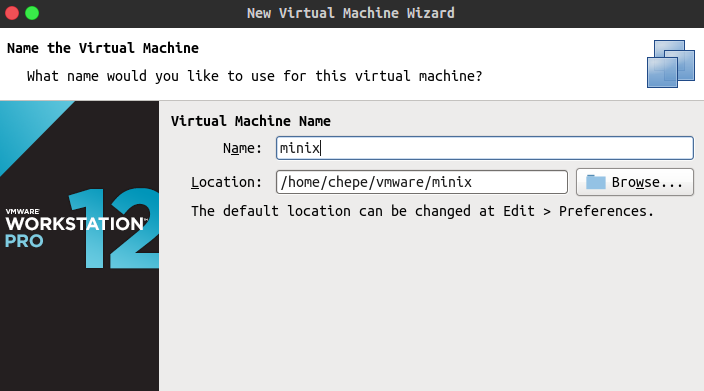
\includegraphics[width=0.6\textwidth]{vm/min04.png}
  \caption{Ruta de creación de máquina}
\end{figure}

Indicar el tamaño del disco duro (se recomienda crear disco de 2GB).
\begin{figure}[H]
  \centering
  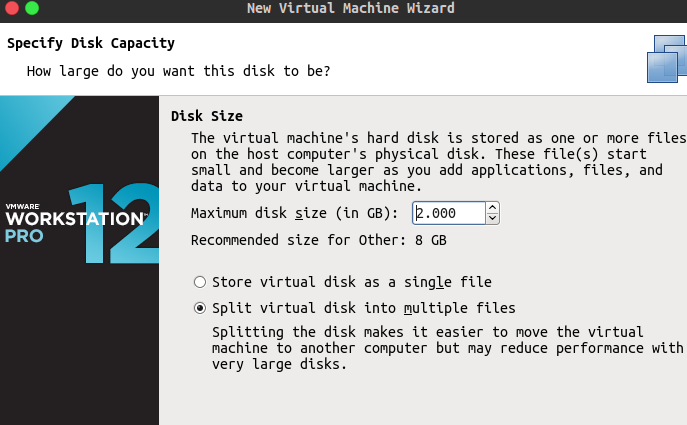
\includegraphics[width=0.6\textwidth]{vm/min05.png}
  \caption{Tamaño de disco duro}
\end{figure}

Seleccionar la opción \textit{Customize Hardware...}.
\begin{figure}[H]
  \centering
  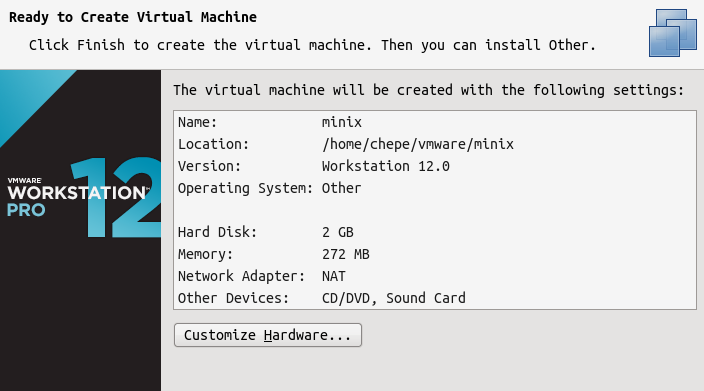
\includegraphics[width=0.6\textwidth]{vm/min10.png}
  \caption{Vista de configuraciones}
\end{figure}

Aumentar el tamaño de la memoria RAM a 512 MB.
\begin{figure}[H]
  \centering
  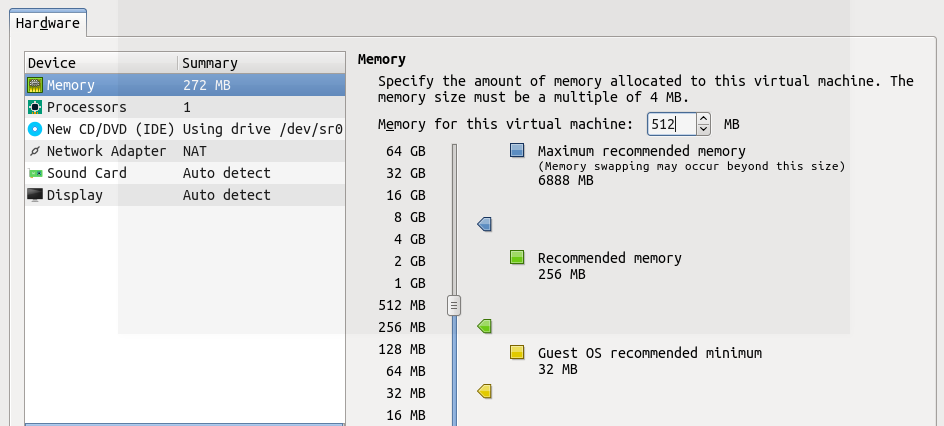
\includegraphics[width=0.6\textwidth]{vm/min11.png}
  \caption{Configuraciones de \textit{Hardware}}
\end{figure}

Terminar creación de máquina virtual, seleccionar opción \textit{Edit virtual machine settings}.
\begin{figure}[H]
  \centering
  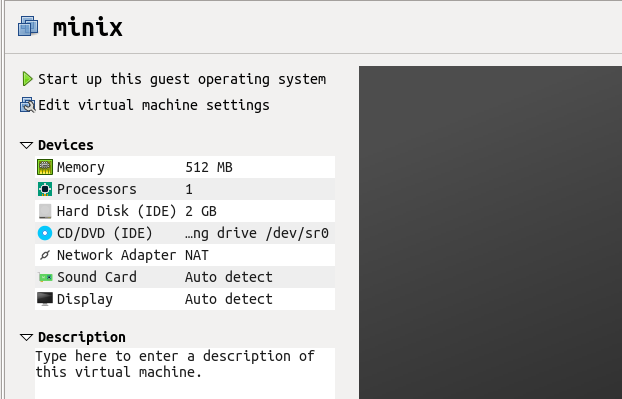
\includegraphics[width=0.6\textwidth]{vm/min13.png}
  \caption{Vista de máquina virtual}
\end{figure}

Dentro de las opciones del dispositivo CD/DVD, seleccionar \textit{Use ISO image} y elegir la imagen ISO previamente descargada de \texttt{Minix 3}.
\begin{figure}[H]
  \centering
  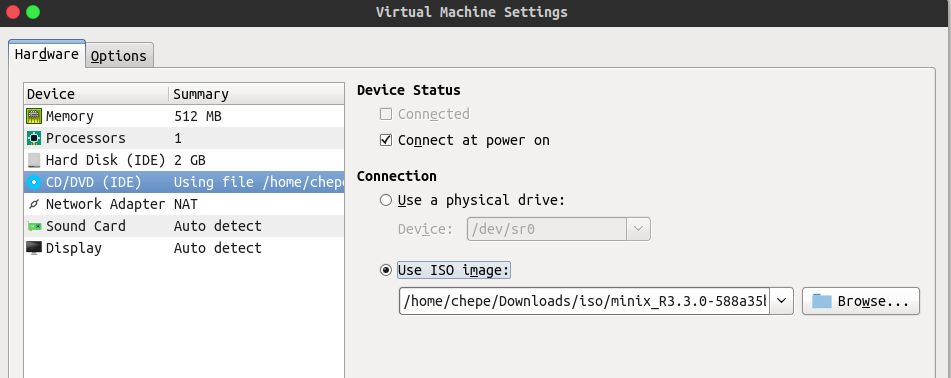
\includegraphics[width=0.6\textwidth]{vm/min14.png}
  \caption{Configuraciones de máquina virtual}
\end{figure}

Prender máquina y comenzar con la instalación del sistema operativo \ref{instalacion}.\\

Una vez instalado el sistema operativo, apagar máquina, ingresar a las configuraciones del sistema operativo, modificar opciones del dispositivo CD/DVD y seleccionar la opción \textit{Use a physical drive}.

\begin{figure}[H]
  \centering
  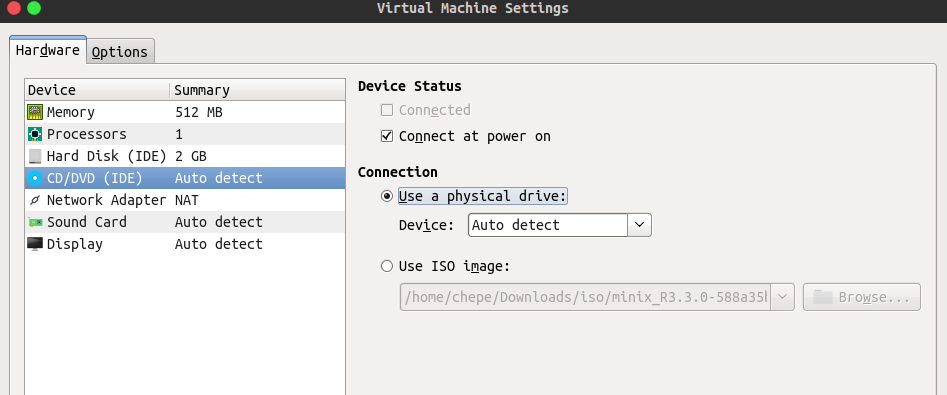
\includegraphics[width=0.6\textwidth]{vm/min32.png}
  \caption{Configuraciones de máquina virtual}
\end{figure}

Al prender la máquina se podra ingresar al sistema operativo ya instalado iniciando sesión como el usuario \texttt{root}.
\begin{figure}[H]
  \centering
  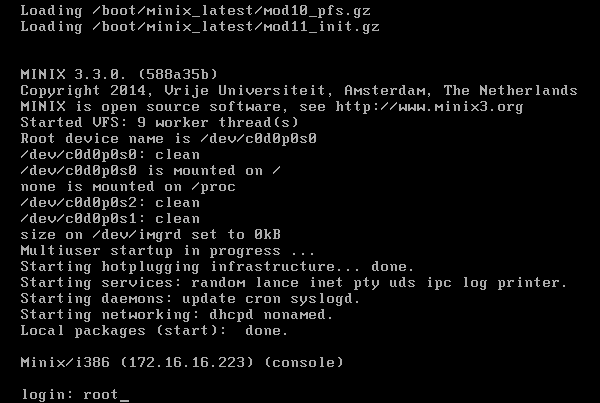
\includegraphics[width=0.6\textwidth]{vm/min33.png}
  \caption{Inicio de sesión}
\end{figure}

\section{VirtualBox}

\subsection*{Preparación de la máquina virtual}
\subsubsection*{...}

\subsection*{Inicio del sistema}
\subsubsection*{...}

\subsection*{Instalación}
\subsubsection*{...}

\subsection*{Verificación}
\subsubsection*{...}


\section{Instalación de sistema operativo}\label{instalacion}

Seleccionar la primera opción que se muestra al prender la máquina para iniciar la instalación del sistema.
\begin{figure}[H]
  \centering
  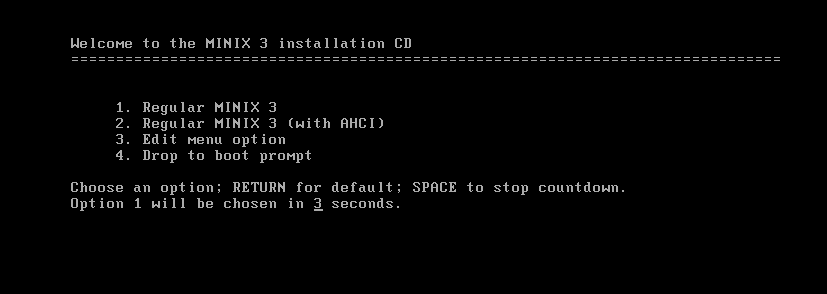
\includegraphics[width=0.7\textwidth]{vm/min15.png}
  \caption{Opciones de inicio}
\end{figure}

Iniciar sesión como el usuario \texttt{root}.
\begin{figure}[H]
  \centering
  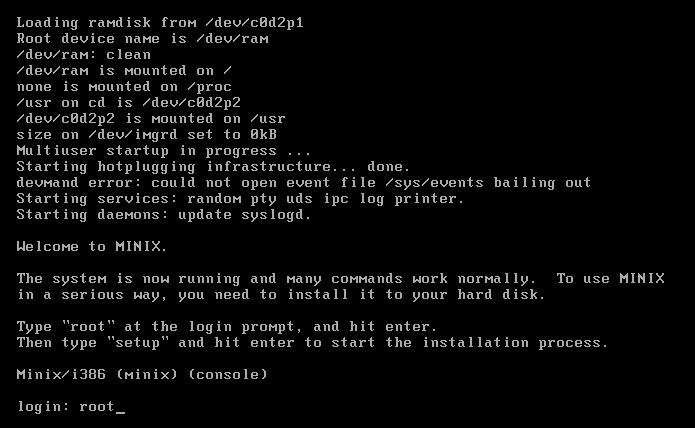
\includegraphics[width=0.7\textwidth]{vm/min16.png}
  \caption{Inicio de sesión}
\end{figure}

Proceder con la instalación ingresando el comando \texttt{setup}.
\begin{figure}[H]
  \centering
  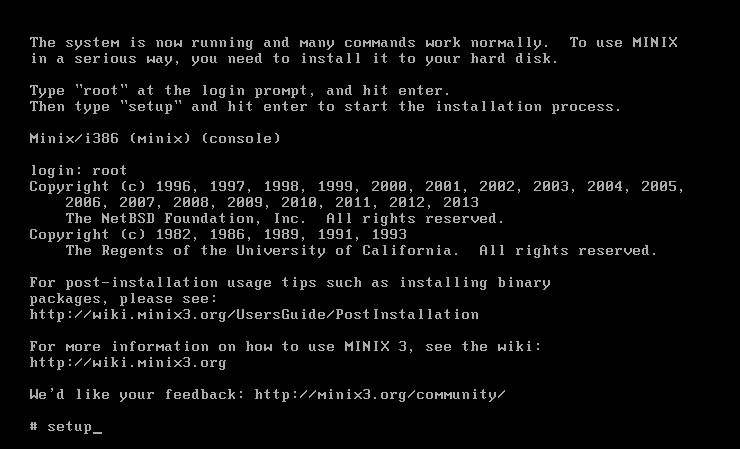
\includegraphics[width=0.7\textwidth]{vm/min18.png}
  \caption{Inicio de instalación}
\end{figure}

Escoger el tipo de teclado a utilizar, en este caso se seleccionó la opción \texttt{latin-america}.
\begin{figure}[H]
  \centering
  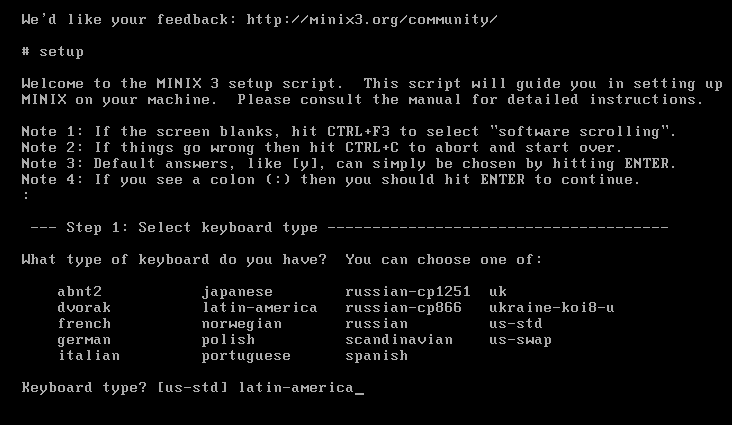
\includegraphics[width=0.7\textwidth]{vm/min19.png}
  \caption{Selección de tipo de teclado}
\end{figure}

Crear la partición para la instalación de sistema operativo, en este caso se escogió el modo automático al presionar la tecla \texttt{[ENTER]}.
\begin{figure}[H]
  \centering
  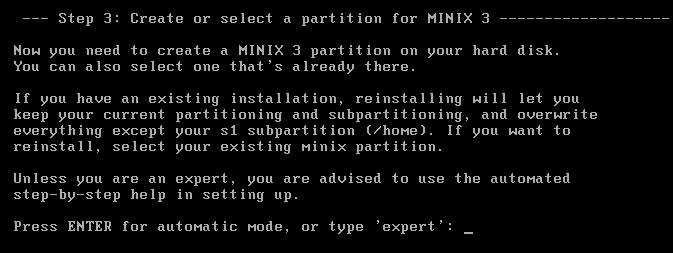
\includegraphics[width=0.7\textwidth]{vm/min20.png}
  \caption{Creación de partición}
\end{figure}

Seleccionar el único disco disponible para la instalación.
\begin{figure}[H]
  \centering
  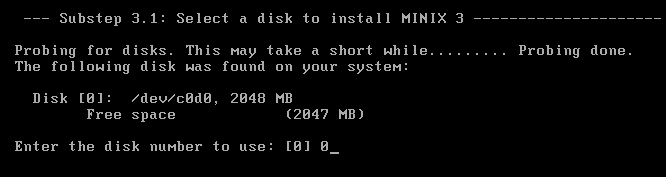
\includegraphics[width=0.7\textwidth]{vm/min21.png}
  \caption{Selección de disco}
\end{figure}

Confirmar las opciones seleccionadas ingresando la palabra \texttt{yes}.
\begin{figure}[H]
  \centering
  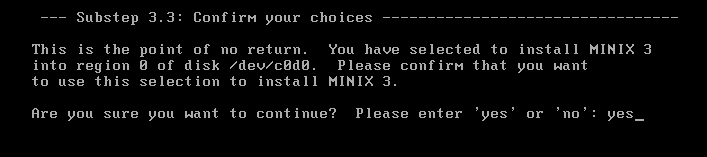
\includegraphics[width=0.7\textwidth]{vm/min22.png}
  \caption{Confirmacion de opciones}
\end{figure}

Indicar cuál será el tamaño de \texttt{/home}.
\begin{figure}[H]
  \centering
  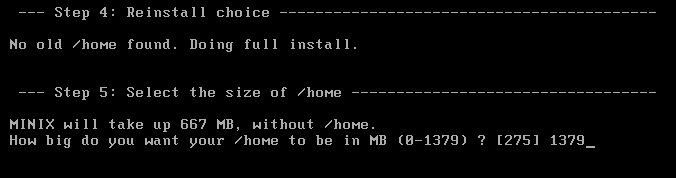
\includegraphics[width=0.7\textwidth]{vm/min24.png}
  \caption{Configuración de tamaño de \texttt{/home}}
\end{figure}

Seleccionar cuál será el tamaño de los bloques, en este caso se dejó el tamaño por defecto de 4KB.
\begin{figure}[H]
  \centering
  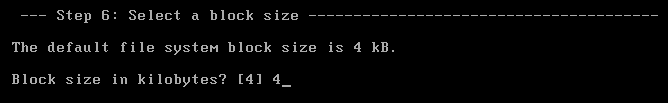
\includegraphics[width=0.7\textwidth]{vm/min26.png}
  \caption{Selección de tamaño de bloques}
\end{figure}

Seleccionar el tipo de tarjeta de red en uso, en este caso se escogió la opción número 9.
\begin{figure}[H]
  \centering
  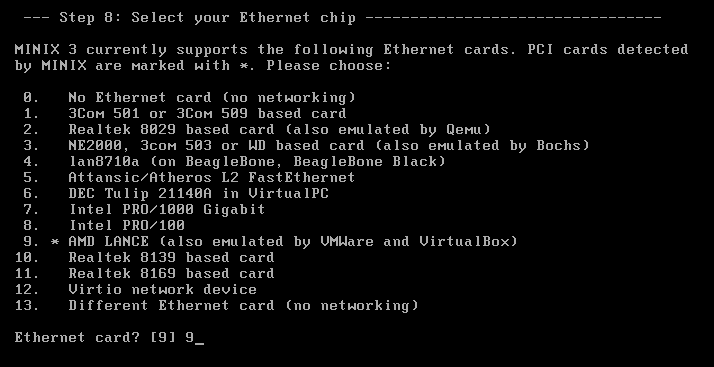
\includegraphics[width=0.7\textwidth]{vm/min27.png}
  \caption{Selección del tipo de tarjeta de red}
\end{figure}

Indicar que se utilice el protocolo \texttt{DHCP} para la configuración automática de la interfaz de red.
\begin{figure}[H]
  \centering
  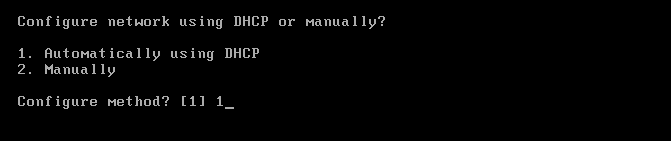
\includegraphics[width=0.7\textwidth]{vm/min30.png}
  \caption{Selección de modo de configuración de interfaz de red}
\end{figure}

Apagar máquina con el comando \texttt{poweroff} y reiniciarla siguiendo las instrucciones del virtualizador correspondiente.
\begin{figure}[H]
  \centering
  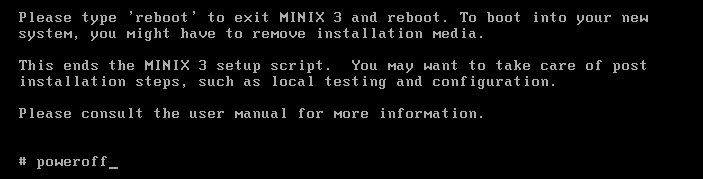
\includegraphics[width=0.7\textwidth]{vm/min31.png}
  \caption{Apagado de la máquina}
\end{figure}

\end{document}
